\section{Validation}
% INTENT: three legs. (1) the suite: 301 tests, every example config driven end
% to end as a registry-drift guard, the editor covered headless. (2) synthetic
% media: what it is, what it deliberately is not (no physical gas model), and
% why publishing it matters more than a field frame would. (3) the measurements
% below, every one of which regenerates with `make bench`.

\begin{figure}[t]
  \centering
  \begin{subfigure}[t]{0.32\textwidth}
    
\includegraphics[width=\textwidth]{figures/plume-source.png}
    \caption{source frame}
  \end{subfigure}\hfill
  \begin{subfigure}[t]{0.32\textwidth}
    
\includegraphics[width=\textwidth]{figures/plume-roi.png}
    \caption{\texttt{static\_mask}: the region of interest}
  \end{subfigure}\hfill
  \begin{subfigure}[t]{0.32\textwidth}
    
\includegraphics[width=\textwidth]{figures/plume-subtracted.png}
    \caption{after \texttt{mean\_background}}
  \end{subfigure}

  \vspace{3mm}
  \begin{subfigure}[t]{0.32\textwidth}
    
\includegraphics[width=\textwidth]{figures/plume-motion-mask.png}
    \caption{\texttt{farneback} thresholded}
  \end{subfigure}\hfill
  \begin{subfigure}[t]{0.32\textwidth}
    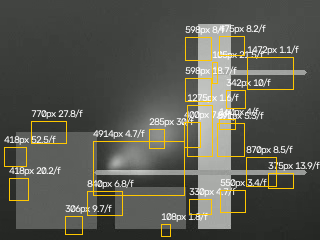
\includegraphics[width=\textwidth]{figures/plume-objects.png}
    \caption{\texttt{motion\_objects}, untuned for this scene}
  \end{subfigure}\hfill
  \caption{The \texttt{baseline} and \texttt{motion} recipes on the synthetic
    plume clip, frame 400. Every panel is a tap out of a real run.}
  \label{fig:plume}
\end{figure}

\begin{figure}[t]
  \centering
  \begin{subfigure}[t]{0.24\textwidth}
    
\includegraphics[width=\textwidth]{figures/geom-edges.png}
    \caption{\texttt{canny}}
  \end{subfigure}\hfill
  \begin{subfigure}[t]{0.24\textwidth}
    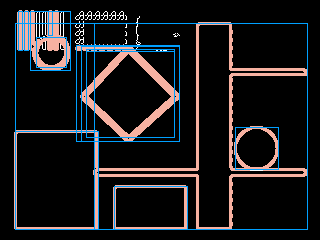
\includegraphics[width=\textwidth]{figures/geom-contours.png}
    \caption{\texttt{contours}}
  \end{subfigure}\hfill
  \begin{subfigure}[t]{0.24\textwidth}
    
\includegraphics[width=\textwidth]{figures/geom-lines.png}
    \caption{\texttt{hough\_lines}}
  \end{subfigure}

  \vspace{3mm}
  \begin{subfigure}[t]{0.24\textwidth}
    
\includegraphics[width=\textwidth]{figures/geom-hog.png}
    \caption{\texttt{hog}}
  \end{subfigure}\hfill
  \begin{subfigure}[t]{0.24\textwidth}
    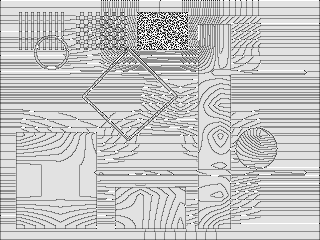
\includegraphics[width=\textwidth]{figures/geom-lbp.png}
    \caption{\texttt{lbp}}
  \end{subfigure}
  \caption{The structure and texture families on the synthetic geometry still.
    A drifting plume gives these operators nothing to describe, which is why
    the scene exists.}
  \label{fig:geometry}
\end{figure}

\begin{table}[t]
  \centering
  \small
  \caption{End-to-end throughput, sinks included, median of three runs on one
    core of an AMD Ryzen 5 5600X. No GPU is used.}
  \label{tab:throughput}
  \begin{tabular}{@{}llrrr@{}}
    \toprule
    Recipe & Resolution & Frames & ms/frame & fps \\
    \midrule
    \inputrows{generated/bench-throughput.tex}
    \bottomrule
  \end{tabular}
\end{table}

\begin{table}[t]
  \centering
  \small
  \caption{Where one frame's budget goes in the \texttt{\BenchCostConfig{}}
    recipe at $320\times240$, sinks excluded.}
  \label{tab:stagecost}
  \begin{tabular}{@{}lrr@{}}
    \toprule
    Stage & ms & \% of frame \\
    \midrule
    \inputrows{generated/bench-stagecost.tex}
    \bottomrule
  \end{tabular}
\end{table}

\begin{figure}[t]
  \centering
  \begin{tikzpicture}
    \begin{axis}[
      width=0.68\textwidth, height=6.2cm,
      xlabel={pixels per frame}, ylabel={frames per second},
      xmode=log, ymode=log, log basis x=10, log basis y=10,
      grid=both, major grid style={rule}, minor grid style={rule!40},
      xmin=6e4, xmax=1.1e6,
      legend style={draw=rule, font=\small, at={(1.03,1)}, anchor=north west},
      tick label style={color=muted}, label style={color=ink},
      cycle list={{accent}, {green}, {amber}, {violet}, {muted}, {ink}},
    ]
      \foreach \column/\label in {baseline/baseline, gasvid/gasvid1,
                                  mog/mog2\_contours, motion/motion,
                                  structure/structure, texture/texture} {
        \addplot+[mark=*, thick] table[x=pixels, y=\column] {generated/bench-sweep.dat};
        \addlegendentryexpanded{\texttt{\label}}
      }
      % 15 fps: the frame rate of the field footage this project started from.
      \addplot[dashed, amber, thick, forget plot, domain=6e4:1.1e6] {15};
    \end{axis}
  \end{tikzpicture}
  \caption{Throughput against frame size, both axes logarithmic. The dashed
    line is 15~fps, the frame rate of the field footage this project started
    from: every video recipe clears it at $320\times240$, and the motion chain
    stops clearing it before $1280\times720$. \texttt{structure} and
    \texttt{texture} describe a single still, so their figure is images per
    second, not a rate they have to keep up with.}
  \label{fig:sweep}
\end{figure}
